\documentclass[10pt,letterpaper,twocolumn]{article}

\usepackage[T1]{fontenc}
\usepackage{lmodern}
\usepackage[margin=0.62in,columnsep=0.27in]{geometry}
\usepackage{amsmath,amssymb,mathtools,bm}
\usepackage{array,booktabs,tabularx}
\usepackage{graphicx}
\usepackage{xcolor}
\usepackage{enumitem}
\usepackage{microtype}
\usepackage{listings}
\usepackage{tikz}
\usetikzlibrary{arrows.meta,positioning}
\usepackage{fancyhdr}
\usepackage{hyperref}

\graphicspath{%
  {figures/}%
  {MATH/paper_facing/paper_V_high_u_gkba/pedagogical/figures/}%
}

% The user-local tools/array package is newer than the available LaTeX kernel.
% Supply the text-mode box fallback expected by that package.
\makeatletter
\def\vcenter@text{\vbox}
\makeatother

\definecolor{navy}{HTML}{17365D}
\definecolor{blue}{HTML}{2B6CB0}
\definecolor{pale}{HTML}{F3F7FB}
\definecolor{paleblue}{HTML}{EAF2FA}
\definecolor{green}{HTML}{2F6B4F}
\definecolor{palegreen}{HTML}{EDF7F1}
\definecolor{brick}{HTML}{9B2C2C}
\definecolor{palered}{HTML}{FFF1F1}
\definecolor{muted}{HTML}{4A5568}
\definecolor{codebg}{HTML}{F6F8FA}

\hypersetup{
  colorlinks=true,
  linkcolor=navy,
  urlcolor=blue,
  pdftitle={What We Actually Built: A State-Vector and Matrix Trace of the Holstein-Dimer Stability Diagnosis},
  pdfauthor={Paper V working calculation}
}

\pagestyle{fancy}
\fancyhf{}
\fancyhead[L]{\footnotesize Holstein-dimer stability diagnosis}
\fancyhead[R]{\footnotesize Equations, diagnosis, and correction}
\fancyfoot[C]{\thepage}
\renewcommand{\headrulewidth}{0.3pt}

\setlength{\parindent}{0pt}
\setlength{\parskip}{3.1pt plus 0.5pt}
\setlist{nosep,leftmargin=*,topsep=2pt}
\renewcommand{\arraystretch}{1.12}
\newcolumntype{Y}{>{\raggedright\arraybackslash}X}

\lstdefinestyle{pythontrace}{
  language=Python,
  basicstyle=\ttfamily\fontsize{7.15}{7.75}\selectfont,
  keywordstyle=\color{blue}\bfseries,
  commentstyle=\color{green},
  stringstyle=\color{brick},
  backgroundcolor=\color{codebg},
  frame=single,
  rulecolor=\color{navy!35},
  numbers=left,
  numberstyle=\tiny\color{muted},
  numbersep=5pt,
  xleftmargin=13pt,
  framexleftmargin=10pt,
  columns=fullflexible,
  keepspaces=true,
  showstringspaces=false,
  breaklines=true,
  breakatwhitespace=true,
  postbreak=\mbox{\textcolor{muted}{\(\hookrightarrow\)}\space},
  aboveskip=4pt,
  belowskip=4pt
}

\newcommand{\R}{\mathbb R}
\newcommand{\C}{\mathbb C}
\newcommand{\I}{\mathbb I}
\newcommand{\ii}{\mathrm i}
\newcommand{\code}[1]{\texttt{#1}}

\newcommand{\tracebox}[3]{%
  \par\smallskip
  \noindent\begin{minipage}{\columnwidth}
    {\color{#1}\rule{\columnwidth}{1.1pt}}\par\vspace{-1pt}
    \small\textbf{\color{#1}#3}\par\smallskip\color{black}
}
\newcommand{\closetracebox}{%
  \par\vspace{1pt}{\color{navy!35}\rule{\columnwidth}{0.35pt}}
  \end{minipage}\par\smallskip
}

\newcommand{\segmenthead}[1]{%
  \par\medskip{\color{navy}\large\bfseries #1}\par
  \vspace{-2pt}{\color{navy}\rule{\columnwidth}{0.7pt}}\par\smallskip
}

\begin{document}

\twocolumn[
\begin{center}
  {\color{navy}\LARGE\bfseries What We Actually Built}\par\vspace{3pt}
  {\Large A State-Vector and Matrix Trace of the Holstein-Dimer Stability Diagnosis}\par\vspace{6pt}
  {\large State space, coordinate embedding, and executable map}\par\vspace{5pt}
  {\small Paper V working calculation, updated 1 August 2026}
\end{center}
\vspace{3pt}
\hrule
\vspace{7pt}
]

\noindent\textbf{Abstract.}
The matrix moment equations for a driven two-site Holstein dimer were reduced
directly to 31 real coordinates and integrated in the pinned strong-coupling
case.  The uncorrected bosonic moment matrix \(M_{\rm B}\) acquired a negative
eigenvalue at \(t=1.48695622\,t_{\rm hop}^{-1}\), before the previously observed
amplitude divergence near \(t=130.47\,t_{\rm hop}^{-1}\).  A first
phonon-energy-neutral barrier corrected only \(\dot N\) and \(\dot A\).  It kept
\(M_{\rm B}\) positive but allowed the electronic density \(\rho\) to reach its
positive-semidefinite boundary at
\(t=120.03094613258\,t_{\rm hop}^{-1}\).  The revised correction acts jointly
on the three independent entries of \(\dot\rho\) and the ten independent
entries of \((\dot N,\dot A)\).  One minimum-norm solve enforces
\(\rho\succeq0\), \(\I_2-\rho\succeq0\), and \(M_{\rm B}\succeq0\), while its
electronic lift preserves \(\operatorname{tr}\rho=1\) and its full energy row
sets the correction's instantaneous internal-energy flux to zero.  A fresh adaptive
trajectory reached \(t=1000\,t_{\rm hop}^{-1}\) with all three matrix
conditions satisfied, \(\max_j|x_j|\le1.942\), and no nonconverged sampled
barrier solve.  This establishes long-horizon stabilization for the pinned
protocol.  Step refinement at the long horizon and additional
representability conditions remain further tests.

\tracebox{navy}{paleblue}{Reading route: main argument first, appendices on demand}
Read Sections~0, 1, 1A, 1B, 2, and 3 in that order.  They form the complete
derivation from the archive equations to the 31-coordinate trajectory and its
joint correction; a first reading can stop after Section~3.

Appendices~A1--A2 (pp.~\pageref{app:forensic-derivative}--
\pageref{app:restricted-amplitude}) are a separate forensic branch.  Read them
only to inspect the earlier 13-coordinate transcription audit and its late
amplitude failure.  Appendices~B1--B7 (pp.~\pageref{app:parameters}--
\pageref{app:composition}) are point-of-use references: B1 fixes the pulse and
parameters; B2--B5 expand matrix storage and reconstruction; B6 expands the
five matrix velocities entry by entry; and B7 shows their final composition
into the Python right-hand side.  The main text names the relevant appendix
where each detour becomes useful.
\closetracebox

\segmenthead{0. The problem and the direct calculation}

The five archive equations of Riva, Simoni, and Ping, arXiv:2606.22233,
advance the electronic density \(\rho\), coherent phonon amplitude \(B\),
normal phonon moment \(N\), anomalous phonon moment \(A\), and
electron--phonon correlation \(C\).  Section~1A reproduces Eqs.~(14a)--(14e)
and performs their two-site Holstein specialization.  The resulting
calculation is the following direct reduction and integration:
\[
\boxed{
\begin{gathered}
(\rho,B,N,A,C)=X\ \text{and their matrix equations}\\[-1pt]
\downarrow\ \text{two-site Holstein specialization}\\[-1pt]
X\xrightarrow{\mathcal R}x\in\R^{31},
\qquad X=\mathcal E(x)\\[-1pt]
\downarrow\ \dot x=\Pi F(t,\mathcal E(x))\\[-1pt]
\text{adaptive time trajectory and matrix physicality tests.}
\end{gathered}}
\]
The symbol \(t_{\rm hop}>0\) is the electronic hopping energy.  It is the
energy unit, and \(t_{\rm hop}^{-1}\) is the time unit.

The motivating observation came from the notes titled
\emph{Dynamics on the Hubbard Dimer}.  Their electronic sector is a Hubbard
dimer, and the equations used here attach one local phonon to each site through
the Holstein density--displacement coupling.  The resulting dynamical model is
therefore the two-site Hubbard--Holstein, or Holstein-coupled Hubbard, dimer.
Its restricted trajectory crossed an amplitude threshold near
\(t=130.47\,t_{\rm hop}^{-1}\).  The direct
31-coordinate calculation asks which matrix condition fails before that
event.  It produced the following sequence.
\begin{enumerate}[label=\textbf{\arabic*.}]
  \item The coordinate map was checked against the archive matrix equations;
  the complete 31-coordinate image contains the generated velocity in the
  tested two-site sector.
  \item The uncorrected trajectory reached
  \(\lambda_{\min}(M_{\rm B})=0\) at
  \(t=1.48695622\,t_{\rm hop}^{-1}\).
  \item A bosonic-only matrix barrier kept \(M_{\rm B}\succeq0\), then
  \(\rho\) reached its own boundary at
  \(t=120.03094613258\,t_{\rm hop}^{-1}\).
  \item A joint electronic--bosonic barrier enforced all three matrix
  inequalities through \(t=1000\,t_{\rm hop}^{-1}\).
\end{enumerate}

The earlier 13-coordinate implementation remains useful as a forensic
transcription check in Appendix~A.  It is not an intermediate state required
to construct or run the 31-coordinate model.

\tracebox{brick}{palered}{Result at the original failure horizon}
The earliest detected failure of the uncorrected 31-coordinate dynamics is
bosonic positive-semidefiniteness.  Constraining only that matrix transfers
the next active boundary to the electronic density.  The joint correction
kept \(0\preceq\rho\preceq\I_2\) and \(M_{\rm B}\succeq0\) through the old
amplitude-divergence horizon while preserving trace and adding zero
instantaneous internal-energy flux.  Section~3 derives this correction and states the
measured bounds.
\closetracebox

\segmenthead{1. From the density operator to the stored arrays}

For a pure joint electron--phonon state \(\lvert\Psi(t)\rangle\), the familiar
density-operator construction is
\[
\varrho(t)=\lvert\Psi(t)\rangle\langle\Psi(t)\rvert,
\qquad
\langle O\rangle_t=\operatorname{Tr}[\varrho(t)O].
\]
The operator \(\varrho\) acts on the full electron--phonon Hilbert space.  The
electronic reduced density operator follows by tracing over the phonons,
\[
\varrho_{\rm e}(t)=\operatorname{Tr}_{\rm ph}\varrho(t).
\]
The complete reduction chain is
\[
\boxed{
\varrho
\xrightarrow{\operatorname{Tr}_{\rm ph}}
\varrho_{\rm e}
\xrightarrow{\langle c_j^\dagger c_i\rangle}
\rho.}
\tag{0a}
\]
The first map removes the phonon degrees of freedom and leaves the complete
electronic many-body density operator \(\varrho_{\rm e}\).  The second map
evaluates one creation--annihilation pair.  The operator \(c_i\) annihilates an
electron on site \(i\), \(c_j^\dagger\) creates one on site \(j\), and the
dagger marks the adjoint operation.  For sites \(i,j\in\{0,1\}\),
\[
\rho_{ij}(t)
=\operatorname{Tr}_{\rm e}[\varrho_{\rm e}(t)c_j^\dagger c_i]
=\operatorname{Tr}[\varrho(t)c_j^\dagger c_i].
\]
This \(2\times2\) array is the electronic one-body reduced density matrix
(1-RDM).  The phonon trace produces \(\varrho_{\rm e}\); the further one-body
reduction produces \(\rho\).  Thus \(\rho\) records one-body electronic
occupations and coherences rather than the complete phonon-traced electronic
density operator.  Its diagonal entries are site occupations per spin, and its
off-diagonal entries are electronic coherences between the two sites.  The
compression from \(\varrho\) to \(\rho\) can produce a mixed 1-RDM with
\(\rho^2\neq\rho\), even when \(\varrho=\lvert\Psi\rangle\langle\Psi\rvert\)
is a pure-state projector.  For a single electron with a pure electronic
state, the site-basis 1-RDM reduces to the familiar ket--bra matrix.

For each phonon mode \(q\in\{0,1\}\), begin with its annihilation operator
\(b_q\).  The first phonon moment is its expectation value,
\[
B_q=\langle b_q\rangle,
\qquad
\delta b_q=b_q-B_q.
\tag{1}
\]
For a complex number \(z=a+\ii b\), where \(a,b\in\R\) and
\(\ii^2=-1\), the symbols \(\Re z=a\) and \(\Im z=b\) denote its real and
imaginary parts.  The symbol \(\R\) denotes the real numbers.
The symbol \(\C\) denotes the complex numbers.
Using dimensionless position and momentum quadratures
\[
Q_q=\frac{b_q+b_q^\dagger}{\sqrt2},
\qquad
P_q=\frac{b_q-b_q^\dagger}{\ii\sqrt2},
\]
the mean values are \(\langle Q_q\rangle=\sqrt2\Re B_q\) and
\(\langle P_q\rangle=\sqrt2\Im B_q\).  Thus \(B_q\) carries the coherent
displacement and momentum of phonon mode \(q\).

The centered operator \(\delta b_q\) measures fluctuations around that mean.
A \emph{moment} is an expectation value of a product of operators.  In this
calculation, the two bosonic second moments are
\[
N_{qq'}=\langle\delta b_{q'}^\dagger\delta b_q\rangle,
\qquad
A_{qq'}=\langle\delta b_q\delta b_{q'}\rangle.
\tag{2}
\]
Both \(N\) and \(A\) are second moments of centered phonon operators.
The normal moment \(N\) stores centered occupation on its diagonal and
ordinary cross-mode covariance off diagonal.  The anomalous moment \(A\)
stores two-phonon pair coherence; its real and imaginary parts encode
phase-sensitive quadrature covariance and, together with \(N\), determine
squeezing and its orientation.  For example, \(N_{00}\) is the
centered occupation of mode 0, \(N_{01}\) correlates the two modes, and
\(A_{00}\) measures a same-mode pair fluctuation.

The electronic one-body fluctuation is
\(c_j^\dagger c_i-\rho_{ij}\), and the centered phonon fluctuation is
\(\delta b_q=b_q-B_q\).  Their connected correlation is
\[
C^q_{ij}
=\left\langle
\delta b_q\bigl(c_j^\dagger c_i-\rho_{ij}\bigr)
\right\rangle.
\]
Since \(\langle\delta b_q\rangle=0\) and \(\rho_{ij}\) is a scalar,
\[
C^q_{ij}
=\langle\delta b_q c_j^\dagger c_i\rangle
-\rho_{ij}\langle\delta b_q\rangle
=\langle\delta b_q c_j^\dagger c_i\rangle.
\]
Thus \(C^q_{ij}\) measures how a phonon fluctuation in mode \(q\) co-varies with the
electronic occupation or coherence selected by \((i,j)\).  The connected
construction removes the factorized mean-field contribution already carried
by \(B\) and \(\rho\).  In each matrix slice, \(C^q_{00}\) and \(C^q_{11}\)
couple mode \(q\) to the two site occupations; \(C^q_{01}\) and
\(C^q_{10}\) couple it to the two directed electronic coherences.

An array assigns one complex number to every permitted tuple of indices.  Thus
the correlation tensor is the three-index map
\[
\begin{aligned}
C:\{0,1\}^3&\longrightarrow\C,\\
(q,i,j)&\longmapsto C[q,i,j],
\qquad q,i,j\in\{0,1\}.
\end{aligned}
\]
An \emph{axis} is one position in the input tuple, and the array's
\emph{shape} lists the number of available values along each axis.  Here every
index takes the two values 0 and 1:
\[
\begin{aligned}
B[q]&\longleftrightarrow(2,),\\
\rho[i,j]&\longleftrightarrow(2,2),\\
C[q,i,j]&\longleftrightarrow(2,2,2).
\end{aligned}
\]
The tuple to the right of each arrow is the corresponding shape.
The number of axes is the tensor \emph{order}.  Thus \(B\) is an order-one
tensor or vector; \(\rho\), \(N\), and \(A\) are order-two tensors or
matrices; and \(C\) is an order-three tensor.  In the shape
\((2,2,2)\), the multiplication signs separate axis lengths.  The symbol
\(\otimes\) denotes the distinct operation called a tensor product.

These definitions give the physical roles and array shapes:

\begin{center}
\small
\begin{tabularx}{\columnwidth}{@{}c c Y@{}}
\toprule
object & shape & physical content\\
\midrule
\(\rho\) & \((2,2)\) & electronic site occupation and coherence\\
\(B\) & \((2,)\) & mean phonon amplitude; its real and imaginary parts encode displacement and momentum quadratures\\
\(N\) & \((2,2)\) & centered phonon occupations and ordinary cross-mode correlations\\
\(A\) & \((2,2)\) & same-mode and cross-mode pair or squeezing correlations\\
\(C\) & \((2,2,2)\) & joint phonon--electron fluctuation correlations\\
\bottomrule
\end{tabularx}
\end{center}

The three axes of \(C\) carry one phonon index and two electronic indices:
\[
C[q,i,j]=(C^q)_{ij},
\qquad
C=(C^0,C^1),
\qquad
C^0,C^1\in\C^{2\times2}.
\]
Thus the NumPy shape \((2,2,2)\) is a stack of two electronic matrices,
\[
\begin{aligned}
C[0,:,:]&=C^0=
\begin{pmatrix}C^0_{00}&C^0_{01}\\C^0_{10}&C^0_{11}\end{pmatrix},\\[3pt]
C[1,:,:]&=C^1=
\begin{pmatrix}C^1_{00}&C^1_{01}\\C^1_{10}&C^1_{11}\end{pmatrix}.
\end{aligned}
\]
The first slice records correlations with phonon mode 0; the second records
correlations with phonon mode 1.  Each slice uses its rows and columns for the
two electronic sites.

The unrestricted stack therefore contains
\[
\underbrace{2\cdot2\cdot2}_{q,i,j}=8\ \text{complex entries}
=16\ \text{real entries}.
\]
The tested closure also imposes
\(\operatorname{tr}C^0=\operatorname{tr}C^1\).  This one complex equality is
two real constraints, so \(C\) contributes \(16-2=14\) independent real
coordinates to the 31-coordinate state.  By comparison, an \(8\times8\)
complex matrix has \(8\cdot8=64\) complex entries and only two axes.

Shape specifies the available components.  A \emph{tensor contraction}
specifies how those components combine.  For each mode \(q\), let
\(G_q\in\C^{2\times2}\) be the local electron--phonon coupling matrix.  The
scalar \(g\) is the local Holstein coupling strength.  The dimer uses
\[
G_0=\begin{pmatrix}g&0\\0&0\end{pmatrix},
\qquad
G_1=\begin{pmatrix}0&0\\0&g\end{pmatrix}.
\]
One contraction pattern in the electronic equation forms the matrix
\[
\begin{aligned}
Y
&=\sum_{q=0}^{1}G_qC^q
=G_0C^0+G_1C^1\\
&=\begin{pmatrix}
gC^0_{00}&gC^0_{01}\\
gC^1_{10}&gC^1_{11}
\end{pmatrix}
\in\C^{2\times2}.
\end{aligned}
\]
Its component form shows how an order-three input produces an order-two
output:
\[
Y_{ij}
=\sum_{q=0}^{1}\sum_{k=0}^{1}(G_q)_{ik}C^q_{kj}.
\]
The contraction sums over the mode index \(q\) and the shared electronic index
\(k\).  Those two indices disappear from the output; the unsummed row and
column indices \(i,j\) remain, giving \(Y\) shape \((2,2)\).  Equation~(25)
uses this pattern inside the correlation-feedback matrix \(\Phi\).  Other
contractions sum different indices to produce the shapes required by
\(\dot N\), \(\dot A\), and \(\dot C\).

\segmenthead{1A. From the archive equations to the Holstein dimer}

The differential system can now be written without an external lookup.
Electronic indices \(i,j,k,l\) label one-electron orbitals, and phonon indices
\(q,q'\) label modes.  The Kronecker delta \(\delta_{ij}\) equals one when
\(i=j\) and zero otherwise.  The source uses the longer symbols
\(\delta\rho_{qq'}\), \(\delta\bar\rho_{q'q}\), and
\(\delta\rho^q_{ij}\).  The active notation is the pure renaming
\[
N_{qq'}=\delta\rho_{qq'},\qquad
A_{q'q}=\delta\bar\rho_{q'q},\qquad
C^q_{ij}=\delta\rho^q_{ij}.
\]
The matrices \(g^{q-}\) and \(g^{q+}\) are the source coupling vertices for
phonon annihilation and creation, respectively, and \(\widetilde h\) is the
coherent-phonon-dressed one-electron Hamiltonian.

\tracebox{navy}{paleblue}{Moment closure: why five objects form one ODE}
For any time-independent operator \(O\), the many-body Hamiltonian gives
\[
\frac{d}{dt}\langle O\rangle
=\ii\langle[H,O]\rangle.
\]
Choosing \(O=c_j^\dagger c_i\) generates expectations containing one phonon
operator; centering them produces \(C^q_{ij}\).  Choosing
\(O=\delta b_qc_j^\dagger c_i\) then generates moments containing two phonon
operators and additional electronic operator products.  Repeating the
derivative produces an ascending moment hierarchy:
\[
\rho\longrightarrow C
\longrightarrow
\langle\delta b\,\delta b\,c^\dagger c\rangle,
\ \langle\delta b\,c^\dagger c\,c^\dagger c\rangle
\longrightarrow\cdots .
\]
One moment equation has therefore introduced higher moments.  A
\emph{closure} is the rule that expresses the moments required by these
derivatives through a chosen finite retained set.  The equal-time
second-order closure used here replaces the generated higher moments by
products of the retained objects.  In Eq.~(14d), this factorization appears
explicitly through products such as
\[
(\delta_{qq'}+N_{qq'})(\delta_{il}-\rho_{il})\rho_{kj},
\qquad
N_{qq'}(\delta_{kj}-\rho_{kj})\rho_{il}.
\]
After this approximate replacement, every derivative is a function of
\(X=(\rho,B,N,A,C)\) itself.  The closure has therefore converted the open
hierarchy into the finite approximate matrix vector field
\[
F(t,X)
=\bigl(F_\rho,F_B,F_N,F_A,F_C\bigr)
=\dot X.
\]
Its output has the same five matrix shapes and equality relations as its input.
The resulting finite ODE is self-contained: each retained state produces the
next retained velocity.  Physical moment conditions impose additional matrix
inequalities on the states generated by this finite vector field.
\closetracebox

\textbf{Electronic density, archive Eq.~(14a).}
After relabeling the source's electronic indices as \(i,j,k\),
\[
\begin{aligned}
\dot\rho_{ij}={}&-\ii[\widetilde h,\rho]_{ij}\\
&+\left\{-\ii\sum_q\sum_k
\left[g^{q-}_{ik}C^q_{kj}
+g^{q+}_{ki}(C^q_{jk})^\ast\right]
+\mathrm{H.c.}\right\}.
\end{aligned}
\tag{14a}
\]
Here \(\mathrm{H.c.}\) adds the conjugate transpose of the matrix enclosed in
braces.  The two-site Holstein restriction takes
\[
\begin{aligned}
i,j,k,q&\in\{0,1\},\\
g^{q+}=g^{q-}=G_q&=g\lvert q\rangle\langle q\rvert,\\
\widetilde h&=h(t).
\end{aligned}
\tag{D1}
\]
Consequently the electronic equation becomes
\[
\begin{aligned}
\Phi_{ij}
&=-\ii\sum_{q,k}
\left[(G_q)_{ik}C^q_{kj}
+(G_q)_{ki}(C^q_{jk})^\ast\right]\\
&=-\ii g\left[C^i_{ij}+(C^i_{ji})^\ast\right],\\
\dot\rho&=-\ii[h(t),\rho]+\Phi+\Phi^\dagger.
\end{aligned}
\tag{D14a}
\]

\textbf{Normal phonon moment, archive Eq.~(14b).}
In the active notation, the source equation is
\[
\begin{aligned}
\dot N_{qq'}={}&-\ii(\omega_q-\omega_{q'})N_{qq'}\\
&-\ii\sum_{i,j}
\left[-g^{q'-}_{ij}C^q_{ji}
+g^{q+}_{ij}(C^{q'}_{ji})^\ast\right].
\end{aligned}
\tag{14b}
\]
The dimer tracks one spin channel in \(\rho\) and \(C\); the two identical
spin channels contribute the factor \(\nu=2\) to every purely bosonic
velocity.  With \(\omega_0=\omega_1=\omega_{\rm ph}\) and Eq.~(D1),
\[
\begin{aligned}
\dot N_{qq'}={}&-\ii(\omega_q-\omega_{q'})N_{qq'}\\
&+\ii\nu g C^q_{q'q'}
-\ii\nu g(C^{q'}_{qq})^\ast.
\end{aligned}
\tag{D14b}
\]

\textbf{Anomalous phonon moment, archive Eq.~(14c).}
The general source equation is
\[
\begin{aligned}
\dot A_{q'q}={}&-\ii(\omega_{q'}+\omega_q)A_{q'q}\\
&-\ii\sum_{i,j}
\left[g^{q+}_{ij}C^{q'}_{ij}
+g^{q'+}_{ij}C^q_{ij}\right].
\end{aligned}
\tag{14c}
\]
Locality and the spin sum reduce it to
\[
\dot A_{q'q}
=-\ii(\omega_{q'}+\omega_q)A_{q'q}
-\ii\nu g\left(C^{q'}_{qq}+C^q_{q'q'}\right).
\tag{D14c}
\]

\textbf{Electron--phonon correlation, archive Eq.~(14d).}
This equation transports \(C\) and creates it from \(\rho\), \(N\), and
\(A\):
{\footnotesize
\[
\begin{aligned}
\dot C^q_{ij}={}&-\ii\left(
[\widetilde h,C^q]_{ij}+\omega_qC^q_{ij}\right)\\
&-\ii\sum_{q'}\sum_{k,l}g^{q'+}_{kl}
(\delta_{qq'}+N_{qq'})(\delta_{il}-\rho_{il})\rho_{kj}\\
&+\ii\sum_{q'}\sum_{k,l}g^{q'+}_{kl}N_{qq'}
(\delta_{kj}-\rho_{kj})\rho_{il}\\
&-\ii\sum_{q'}\sum_k g^{q'-}_{jk}A_{q'q}\rho_{ki}
+\ii\sum_{q'}\sum_k g^{q'-}_{kj}A_{q'q}\rho_{ik}.
\end{aligned}
\tag{14d}
\]
}
For the dimer, define the occupied-to-available and
available-to-occupied products
\[
R_{q'}=(\I_2-\rho)G_{q'}^{\mathsf T}\rho,
\qquad
L_{q'}=\rho G_{q'}^{\mathsf T}(\I_2-\rho).
\tag{D2}
\]
The five source matrices obtained by applying Eq.~(D1) to Eq.~(14d) are
{\small
\[
\begin{aligned}
S_0^q&=-\ii R_q,\\
S_1^q&=-\ii\sum_{q'}N_{qq'}R_{q'},\\
S_2^q&=+\ii\sum_{q'}N_{qq'}L_{q'},\\
(S_3^q)_{ij}
&=-\ii\sum_{q',k}(G_{q'})_{jk}A_{q'q}\rho_{ki},\\
(S_4^q)_{ij}
&=+\ii\sum_{q',k}(G_{q'})_{kj}A_{q'q}\rho_{ik}.
\end{aligned}
\tag{D3}
\]
}
Hence the complete dimer correlation equation is
\[
\dot C^q
=-\ii\bigl(h(t)C^q-C^qh(t)+\omega_qC^q\bigr)
+\sum_{a=0}^{4}S_a^q.
\tag{D14d}
\]

\textbf{Coherent phonon amplitude, archive Eq.~(14e).}
The source equation is
\[
\dot B_q
=-\ii\left(\omega_qB_q
+\sum_{i,j}g^{q+}_{ij}\rho_{ij}\right),
\tag{14e}
\]
and its spin-degenerate local reduction is
\[
\dot B_q
=-\ii\left(\omega_qB_q+\nu g\rho_{qq}\right).
\tag{D14e}
\]
The dressed dimer Hamiltonian appearing in Eqs.~(D14a) and (D14d) is
\[
h(t)=
\begin{pmatrix}
V(t)/2&-t_{\rm hop}\\
-t_{\rm hop}&-V(t)/2
\end{pmatrix}
+\sum_{q=0}^{1}G_q(B_q+B_q^\ast).
\tag{D4}
\]
The scalar \(V(t)\) is the driven difference between the two site energies;
Appendix~B1 substitutes the pulse used in the trajectory.  Equations
(D14a)--(D14e) are the five matrix velocities evaluated by the dimer code.
Appendix~B6 is the optional entry-by-entry expansion of these same five
velocities; it is not needed before proceeding to the coordinate reduction.

\segmenthead{1B. From the dimer matrices to the real state vector}

At one time \(t\), the complete matrix state is the single tuple
\[
X(t)=(\rho(t),B(t),N(t),A(t),C^0(t),C^1(t)).
\tag{3}
\]
The ordinary capital \(X(t)\) names one current state.  The calligraphic
symbol \(\mathcal X\), read \emph{script X}, names the set of every tuple with
the same permitted shapes and structural relations.

Let \(\mathcal A_\rho\) be the affine structural space of Hermitian,
unit-trace \(2\times2\) electronic matrices.  Let
\(\operatorname{Herm}(2)\) be the set of Hermitian
\(2\times2\) matrices, satisfying \(N=N^\dagger\), and let
\(\operatorname{Sym}_2(\C)\) be the set of complex-symmetric \(2\times2\)
matrices, satisfying \(A=A^{\mathsf T}\).  Let \(\mathcal C_2\) contain pairs
\((C^0,C^1)\) whose two traces agree.  The Cartesian-product symbol
\(\times\) bundles one choice from each component set.  The operation
\(\operatorname{tr}\) sums the diagonal entries of a finite matrix.  These
definitions give
\[
\begin{aligned}
\mathcal A_\rho
&=\{\rho\in\C^{2\times2}:\rho=\rho^\dagger,
\operatorname{tr}\rho=1\},\\
\operatorname{Herm}(2)
&=\{N\in\C^{2\times2}:N=N^\dagger\},\\
\operatorname{Sym}_2(\C)
&=\{A\in\C^{2\times2}:A=A^{\mathsf T}\},\\
\mathcal C_2
&=\{(C^0,C^1)\in(\C^{2\times2})^2:
\operatorname{tr}C^0=\operatorname{tr}C^1\},\\
\mathcal X
&=\mathcal A_\rho\times\C^2\times\operatorname{Herm}(2)
\times\operatorname{Sym}_2(\C)\times\mathcal C_2.
\end{aligned}
\tag{4}
\]
The factor \(\C^2\) supplies the length-two complex vector \(B\).  Equation
(4) therefore states \(X(t)\in\mathcal X\): one structurally admissible
electronic matrix, one coherent-phonon vector, one structurally admissible
normal-moment matrix, one structurally admissible anomalous-moment matrix, and
one structurally admissible correlation pair.  Its computational purpose is
to specify the input type of the matrix evolution and the structural relations
that its output velocity must preserve.

For any positive integer \(n\), the space \(\R^n\) contains ordered lists of
\(n\) real numbers.  The reduction \(\mathcal R:\mathcal X\to\R^{31}\)
extracts the independent real coordinates, and the block-affine embedding
\(\mathcal E:\R^{31}\to\mathcal X\) reconstructs the matrices.  On the
tested structural sector, \(\mathcal R\circ\mathcal E\) is the identity.
Thus \(x\) and \(X=(\rho,B,N,A,C)\) contain the same independent information:
\(\mathcal R\) changes matrices into coordinates and \(\mathcal E\) changes
those coordinates back into matrices.  Neither map advances physical time.
The matrix vector field \(F\) computes \(\dot X\), and the velocity reduction
\(\Pi=D\mathcal R\) extracts the corresponding 31 real slopes:
\[
x\in\R^{31}
\xrightarrow{\mathcal E}
X\in\mathcal X
\xrightarrow{F(t,\,\cdot\,)}
\dot X
\xrightarrow{\Pi}
\dot x\in\R^{31}.
\tag{5}
\]
Their composition is the real-vector right-hand-side function \(f\).  One
evaluation is
\[
\boxed{\dot x=f(t,x)=\Pi\!\left(F\!\left(t,\mathcal E(x)\right)\right)}.
\tag{6}
\]
Appendix~B7 displays this composition as the final sequence of Python function
calls.  It is most useful after the mathematical maps in Eq.~(6) are clear.

\textbf{Explicit block-affine realization.}
The reduction \(\mathcal R\) records the following independent coordinates,
and \(\mathcal E\) reconstructs the displayed matrices.  The electronic block
uses the population difference \(\Delta n=\rho_{00}-\rho_{11}\):
\[
\begin{aligned}
x_\rho&=(\Delta n,\Re\rho_{01},\Im\rho_{01})\in\R^3,\\
\rho(x_\rho)&=
\begin{pmatrix}
(1+\Delta n)/2&\Re\rho_{01}+\ii\Im\rho_{01}\\
\Re\rho_{01}-\ii\Im\rho_{01}&(1-\Delta n)/2
\end{pmatrix}.
\end{aligned}
\tag{R1}
\]
The coherent and normal phonon blocks are
\[
\begin{aligned}
x_B={}&(\Re B_0,\Im B_0,\Re B_1,\Im B_1)\in\R^4,\\
B(x_B)={}&
\begin{pmatrix}
\Re B_0+\ii\Im B_0\\
\Re B_1+\ii\Im B_1
\end{pmatrix},\\[2pt]
x_N={}&(N_{00},N_{11},\Re N_{01},\Im N_{01})\in\R^4,\\
N(x_N)={}&
\begin{pmatrix}
N_{00}&\Re N_{01}+\ii\Im N_{01}\\
\Re N_{01}-\ii\Im N_{01}&N_{11}
\end{pmatrix}.
\end{aligned}
\tag{R2}
\]
The complex-symmetric anomalous block is
{\small
\[
\begin{aligned}
x_A={}&(\Re A_{00},\Im A_{00},\Re A_{11},\Im A_{11},
\Re A_{01},\Im A_{01})\in\R^6,\\
A(x_A)={}&
\begin{pmatrix}
\Re A_{00}+\ii\Im A_{00}&\Re A_{01}+\ii\Im A_{01}\\
\Re A_{01}+\ii\Im A_{01}&\Re A_{11}+\ii\Im A_{11}
\end{pmatrix}.
\end{aligned}
\tag{R3}
\]
}
For the correlation block, define the shared trace and the three remaining
complex entries in each slice,
\[
\begin{aligned}
s&=\operatorname{tr}C^0=\operatorname{tr}C^1,
&d_q&=C^q_{00}-C^q_{11},\\
u_q&=C^q_{01},
&v_q&=C^q_{10}.
\end{aligned}
\tag{R4}
\]
Then
\[
C^q=
\begin{pmatrix}(s+d_q)/2&u_q\\v_q&(s-d_q)/2\end{pmatrix},
\qquad q\in\{0,1\},
\tag{R5}
\]
and
{\footnotesize
\[
\begin{aligned}
x_C=(&\Re s,\Im s,
\Re d_0,\Im d_0,\Re u_0,\Im u_0,\Re v_0,\Im v_0,\\
&\Re d_1,\Im d_1,\Re u_1,\Im u_1,\Re v_1,\Im v_1)
\in\R^{14}.
\end{aligned}
\tag{R6}
\]
}
Thus the complete reduction is
\[
\boxed{
\begin{aligned}
x=\mathcal R(X)
&=x_\rho\oplus x_B\oplus x_N\oplus x_A\oplus x_C,\\
x&\in\R^{3+4+4+6+14}=\R^{31}.
\end{aligned}}
\tag{R7}
\]
The symbol \(\oplus\) appends the five coordinate blocks in order.  The fixed
one-half terms in Eq.~(R1) make \(\mathcal E\) affine; the remaining block
reconstructions are linear.

\tracebox{navy}{paleblue}{Why the reconstruction loses no retained information}
Each block records exactly the entries left independent by its equality
relations.  Substitution and re-extraction therefore give
\[
\mathcal R_\rho(\rho(x_\rho))=x_\rho,
\qquad
\mathcal R_C(C^0(x_C),C^1(x_C))=x_C,
\]
and the same identity holds for \(B,N,A\).  Appending the five identities
gives
\[
\boxed{\mathcal R(\mathcal E(x))=x.}
\]
The reconstruction changes representation from 31 real coordinates to five
structured complex arrays.  The vector field \(F\) subsequently supplies the
physical time evolution.
\closetracebox

For a code-level reading of this construction, Appendix~B2 names the state
fields, B3 repeats the affine reduction component by component, B4 lists the
exact Python coordinate names, and B5 displays the reconstruction routine.
Those appendices implement Eqs.~(R1)--(R7); they do not introduce another
mathematical model.

\newcommand{\forensicappendix}{%
\segmenthead{Appendix A1. Forensic derivative agreement}
\phantomsection\label{app:forensic-derivative}

The first diagnostic question in Section~0 concerns transcription: when the
restricted scalar code and the independently written matrix code receive the
same physical state, do they assign the same time derivative to every quantity
that both representations store?

The function \(f_{13}(t,x)\) is the handwritten right-hand side of the first
13-real-coordinate implementation.  That shortcut stored three electronic
coordinates, two relative coherent-phonon coordinates, two symmetry-tied
normal moments, and six symmetry-tied electron--phonon correlations.  It set
the anomalous matrix \(A\) to zero.  The map \(\mathcal E_{13}\) converts those
13 numbers into their represented matrices, and \(\Pi_{13}\) reads the same 13
derivative components from the matrix result.  Call the two calculated slope
vectors \(d_{\rm scalar}\) and \(d_{\rm matrix}\):
\[
d_{\rm scalar}=f_{13}(t,x),
\qquad
d_{\rm matrix}=\Pi_{13}F(t,\mathcal E_{13}(x)).
\tag{7}
\]
A residual is the difference between two calculations of the same target.
Define the derivative-parity residual
\[
r_{\parallel}=d_{\rm scalar}-d_{\rm matrix}.
\tag{8}
\]
A derivative is the tangent vector that controls the first-order displacement
from the current state.  Applying each candidate slope for a short interval
\(\Delta t\) gives
\[
\begin{aligned}
x_{\rm scalar}(t+\Delta t)
&=x+\Delta t\,d_{\rm scalar}+O(\Delta t^2),\\
x_{\rm matrix}(t+\Delta t)
&=x+\Delta t\,d_{\rm matrix}+O(\Delta t^2).
\end{aligned}
\]
Writing their difference as
\(\delta x=x_{\rm scalar}-x_{\rm matrix}\), subtraction gives
\[
\delta x(t+\Delta t)
=\Delta t\,r_{\parallel}+O(\Delta t^2).
\]
Equality of the two derivative vectors therefore means that both
representations predict the same local motion from the same physical state.
This is a \emph{representation-consistency} or \emph{commuting-map} test: on
the shared coordinates, evaluating the handwritten scalar right-hand side
agrees with reconstructing the matrices, evaluating their equations, and
projecting the result back.
Its 13 entries compare the two slope vectors component by component.

For a concrete checked state, start from the Hartree--Fock/zero-correlation
coordinate \(x_0\), take the first-order state
\(x=x_0+10^{-3}f_{13}(0,x_0)\), and evaluate at \(t=10^{-3}\).  Both routes
give
{\footnotesize
\[
\begin{aligned}
d_{\rm scalar}=d_{\rm matrix}=(&0,-0.000375000,
-0.000785398,0,\\
&0,0.000375000,-0.000375000,\\
&-0.000382733,-0.153093109,0,\\
&-0.306186218,-0.000000481,\\
&-0.000765466).
\end{aligned}
\tag{9}
\]
}
Here \(j\in\{0,\ldots,12\}\) labels a stored component.  The measured maximum
component is
\[
\max_j |(r_{\parallel})_j|=9.11\times10^{-18}.
\]
This is floating-point roundoff.  For scale, opposite slopes \(-0.153\) and
\(+0.153\) in one slot would produce a residual of \(-0.306\), revealing a
sign transcription error.

To measure the omitted part, reconstruct the matrix velocity represented by
the 13 retained slopes and subtract it from the full matrix velocity.  The
linear map \(D\mathcal E_{13}(x)\) converts a 13-number slope into the
matrix-shaped velocity generated by those 13 stored directions:
\[
r_{\perp}
=F(t,\mathcal E_{13}(x))
-D\mathcal E_{13}(x)\,[d_{\rm matrix}].
\tag{10}
\]
At the state used in Eq.~(9), two omitted slopes are already present:
\[
\lVert\dot A\rVert_{\rm omitted}=7.50\times10^{-4},
\qquad
|\dot B_{\rm center}|=1.224744871.
\tag{11}
\]
The first is the generated anomalous phonon field.  The second is a uniform
coherent displacement; in the symmetric dimer its electronic Hamiltonian
contribution is proportional to the identity.  The anomalous slope changes
the bosonic fluctuation state and is essential for the physicality test below.

\tracebox{navy}{paleblue}{The two measured residual outcomes}
The retained-coordinate residual \(r_{\parallel}\) is roundoff-level, so the
two implementations agree on all 13 shared derivatives.  The closure residual
\(r_{\perp}\) is nonzero and contains the omitted slopes in Eq.~(11), so the
13-coordinate state fails to contain its full matrix velocity.
\closetracebox

\begin{center}
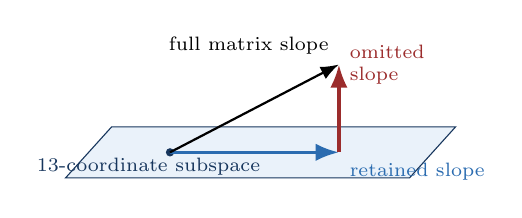
\begin{tikzpicture}[x=0.78cm,y=0.72cm,>=Latex]
  \fill[paleblue] (-3.2,-0.45) -- (2.4,-0.45) -- (3.15,0.45) -- (-2.45,0.45) -- cycle;
  \draw[navy] (-3.2,-0.45) -- (2.4,-0.45) -- (3.15,0.45) -- (-2.45,0.45) -- cycle;
  \coordinate (p) at (-1.5,0);
  \fill[navy] (p) circle (1.5pt);
  \draw[->,very thick,blue] (p) -- (1.25,0) node[below right,font=\scriptsize] {retained slope};
  \draw[->,very thick,brick] (1.25,0) -- (1.25,1.55) node[right,font=\scriptsize,align=left] {omitted\\slope};
  \draw[->,thick,black] (p) -- (1.25,1.55) node[above left,font=\scriptsize] {full matrix slope};
  \node[font=\scriptsize,navy] at (-1.85,-0.25) {13-coordinate subspace};
\end{tikzpicture}
\end{center}

The 31-coordinate state stores every generated matrix direction found in the
tested two-site sector.  For that enlarged state, both
\(r_{\parallel}\) and \(r_{\perp}\) are below \(3\times10^{-14}\) across
the randomized closure tests.

\segmenthead{Appendix A2. The restricted amplitude reproduction}
\phantomsection\label{app:restricted-amplitude}

The plotted quantity \(\max_j|x_j(t)|\) selects the largest absolute component
of the 13-number state at each time.  It records the overall amplitude scale
without choosing one component in advance.

\begin{center}
\includegraphics[width=\columnwidth]{trajectory_max_abs.pdf}

\parbox{0.96\columnwidth}{\scriptsize
\textbf{Strong/weak trajectory comparison.}
The strong-coupling trace reaches the declared \(10^4\) threshold near
\(t=130.47\,t_{\rm hop}^{-1}\); the matched weak-coupling trace remains below
one through \(t=140\,t_{\rm hop}^{-1}\).}
\end{center}

This comparison motivated the diagnostic sequence in Section~0.  Equation~(9)
and the in-plane/out-of-plane diagram then answer a different question: the
two implementations assign the same retained slope, and the full matrix slope
also leaves the old coordinate slice.

}% end \forensicappendix

\segmenthead{2. Uncorrected moments, the positive cone, and the first barrier}

Recall the two \(2\times2\) moment matrices from Eq.~(2):
\(N=(N_{qq'})\) stores normal moments and \(A=(A_{qq'})\) stores anomalous
moments.  Their structural relations are \(N=N^\dagger\) and
\(A=A^{\mathsf T}\).  Let \(\I_2\) denote the \(2\times2\) identity matrix;
\({}^{\mathsf T}\) transposes a matrix, \({}^\ast\) conjugates each entry, and
\({}^\dagger\) performs both operations.

Collect the two centered creation operators and two centered annihilation
operators into the four-entry column vector
\[
\xi=(\delta b_0^\dagger,\delta b_1^\dagger,
      \delta b_0,\delta b_1)^{\mathsf T}.
\]
The row \(\xi^\dagger\) is its conjugate transpose.  Every entry of
\(\langle\xi\xi^\dagger\rangle\) is therefore a second moment.  Grouping the
creation and annihilation entries into \(2\times2\) blocks gives
\[
M_{\rm B}=\langle\xi\xi^\dagger\rangle
=\begin{pmatrix}N^{\mathsf T}&A^\ast\\A&\I_2+N\end{pmatrix}.
\tag{12}
\]
For every complex four-vector \(z\), define the operator-valued linear
combination
\[
O(z)=z^\dagger\xi.
\]
The object \(O(z)\) is an operator on the electron--phonon state space.  Its
product \(O(z)O(z)^\dagger\) is a positive operator, and its expectation value
is the nonnegative scalar
\[
\begin{aligned}
z^\dagger M_{\rm B}z
&=\langle O(z)O(z)^\dagger\rangle\\
&=\lVert O(z)^\dagger\lvert\Psi\rangle\rVert_2^2\geq0.
\end{aligned}
\tag{13}
\]
Thus a physical pair \((N,A)\) produces a positive-semidefinite matrix,
written \(M_{\rm B}\succeq0\).  Equivalently, all four eigenvalues of
\(M_{\rm B}\) are nonnegative.

For \(X=\mathcal E(x)\), let \(\rho_x\) denote its electronic matrix and let
\(M_{{\rm B},x}\) denote Eq.~(12) assembled from its \(N\) and \(A\) blocks.
The coordinates that pass the tested necessary representability conditions
form the subset
\[
\boxed{
\mathcal P=
\{x\in\R^{31}:
\rho_x\succeq0,\ \I_2-\rho_x\succeq0,\
M_{{\rm B},x}\succeq0\}
\subset\R^{31}.}
\tag{13b}
\]
The ambient space \(\R^{31}\) contains every structurally valid coordinate
tuple produced by the reduction.  The subset \(\mathcal P\) contains the
tuples satisfying the tested necessary quantum-moment inequalities.  The
finite equations can still evaluate \(f(t,x)\) for \(x\notin\mathcal P\);
such coordinates violate at least one necessary condition for representing
physical quantum moments.

The positive-semidefinite cone is the fixed admissible set
\[
\mathcal K_d
=\{M\in\C^{d\times d}:M=M^\dagger,\ M\succeq0\}.
\]
Scaling any member by a nonnegative number keeps it in the set, which gives
the set its cone geometry.  The set \(\mathcal K_d\) does not move in time;
the time-dependent matrix \(M_{\rm B}(t)\) is the trajectory moving through
it.  The boundary is reached when the smallest eigenvalue is zero.

Let \(v(t)\) be a normalized eigenvector of a simple smallest eigenvalue,
\(v^\dagger v=1\) and \(M(t)v=\lambda_{\min}(t)v\).  From
\(M(t+\Delta t)=M(t)+\Delta t\,\dot M(t)+O(\Delta t^2)\), first-order
eigenvalue perturbation gives
\[
\lambda_{\min}(t+\Delta t)
=\lambda_{\min}(t)
+\Delta t\,v^\dagger\dot M(t)v+O(\Delta t^2).
\tag{13a}
\]
Thus \(v^\dagger\dot Mv\) is the boundary eigenvalue velocity.  If
\(\lambda_{\min}=0\) and this scalar is negative, the next infinitesimal
motion points outside \(\mathcal K_d\).  The full matrix barrier below avoids
relying on one selected \(v\) when the smallest eigenvalue is degenerate.

For one selected mode \(q\), define its normal occupation \(n\) and anomalous
pair moment \(m\) before reducing Eq.~(12):
\[
n=N_{qq}
=\langle\delta b_q^\dagger\delta b_q\rangle,
\qquad
m=A_{qq}
=\langle\delta b_q\delta b_q\rangle.
\]
The corresponding one-mode moment matrix and its positive-semidefinite
conditions are
\[
M_{\rm B}^{(q)}
=\begin{pmatrix}n&m^\ast\\m&n+1\end{pmatrix},
\qquad
n\geq0,
\qquad
n(n+1)\geq|m|^2.
\tag{14}
\]
A check of \(n\geq0\) leaves the coupled condition involving \(m\)
unevaluated.

\begin{center}
\includegraphics[width=\columnwidth]{closed_scalar_physicality.pdf}

\parbox{0.96\columnwidth}{\scriptsize
\textbf{Physicality trajectory for the complete state.}
The horizontal zero line is the positive-semidefinite boundary.  The full
bosonic moment minimum crosses below zero at
\(t=1.48695622\,t_{\rm hop}^{-1}\), long before the late amplitude event in
Appendix~A2.}
\end{center}

The moment test requires every independent entry of \(N\) and \(A\) that the
matrix equations can generate.  Equations~(R2)--(R3) retain those entries.
Consequently the 31-coordinate vector can assemble exactly the same
\(4\times4\) bosonic moment matrix as the structured matrix calculation.

The barrier constrains the velocity used for the next solver step.  Let
\(M(t)\in\operatorname{Herm}(d)\) be the current matrix and \(\dot M(t)\) its
candidate velocity.  The identity \(\I_d\) has the same size as \(M\),
\(h_\star\geq0\) is the desired eigenvalue margin, \(\beta>0\) is the recovery
rate, and \(\kappa\geq0\) requests additional inward velocity.

For one scalar coordinate \(m_{\rm sc}(t)\) and \(\kappa=0\), the model
inequality is
\[
\dot m_{\rm sc}+\beta(m_{\rm sc}-h_\star)\geq0.
\tag{B0}
\]
At the boundary \(m_{\rm sc}=h_\star\), it requires
\(\dot m_{\rm sc}\geq0\).  In the interior it permits downward motion, but no
faster than \(-\beta(m_{\rm sc}-h_\star)\).  The matrix version imposes the
same rule simultaneously in every eigen-direction:
\[
\dot M+\beta(M-h_\star\I_d)-\kappa\I_d\succeq0.
\tag{B1}
\]
When the uncorrected \(\dot M\) violates this inequality, the optimization
adds a structured correction to \(\dot M\).  It does not project, replace, or
overwrite the current matrix \(M(t)\).

Multiplication by the scalar integrating factor \(e^{\beta t}\), followed by
integration from \(t_0\) to \(t\), gives the matrix
variation-of-constants bound
\[
\begin{aligned}
M(t)\succeq{}&e^{-\beta(t-t_0)}M(t_0)\\
&+\left(h_\star+\frac{\kappa}{\beta}\right)
\left(1-e^{-\beta(t-t_0)}\right)\I_d.
\end{aligned}
\tag{B2}
\]
For \(\kappa=0\), an initial condition
\(M(t_0)\succeq h_\star\I_d\) therefore implies
\(M(t)\succeq h_\star\I_d\), or
\(\lambda_{\min}(M(t))\geq h_\star\).  A positive \(h_\star\) gives a strict
safety margin; \(h_\star=0\) permits a zero eigenvalue.  The three joint
barriers later substitute \(M=\rho\), \(M=\I_2-\rho\), and
\(M=M_{\rm B}\); their derivatives are \(\dot\rho\), \(-\dot\rho\), and
\(\dot M_{\rm B}\), respectively.

For the first bosonic-only correction, define \(D=\dot M_{\rm B}\).  A vector
\[
\begin{aligned}
w=(&w_{N_{00}},w_{N_{11}},w_{N_R},w_{N_I},
w^R_{A_{00}},w^I_{A_{00}},\\
&w^R_{A_{11}},w^I_{A_{11}},w^R_{A_{01}},w^I_{A_{01}})
\in\R^{10}
\end{aligned}
\]
stores corrections to the independent entries of \((\dot N,\dot A)\).  Its
\emph{structured lift} is the map that places these ten real controls into
the larger matrices while enforcing their dependent entries.  Define the
normal and anomalous velocity corrections \(\Delta N(w)\), \(\Delta A(w)\),
and the bosonic lift \(S_{\rm B}:\R^{10}\to\operatorname{Herm}(4)\) by
\[
\begin{aligned}
\Delta N(w)&=
\begin{pmatrix}
w_{N_{00}}&w_{N_R}+\ii w_{N_I}\\
w_{N_R}-\ii w_{N_I}&w_{N_{11}}
\end{pmatrix},\\[3pt]
\Delta A(w)&=
\begin{pmatrix}
w^R_{A_{00}}+\ii w^I_{A_{00}}&w^R_{A_{01}}+\ii w^I_{A_{01}}\\
w^R_{A_{01}}+\ii w^I_{A_{01}}&w^R_{A_{11}}+\ii w^I_{A_{11}}
\end{pmatrix},\\[3pt]
S_{\rm B}(w)&=
\begin{pmatrix}
\Delta N(w)^{\mathsf T}&\Delta A(w)^\ast\\
\Delta A(w)&\Delta N(w)
\end{pmatrix}.
\end{aligned}
\tag{B3}
\]
Although \(S_{\rm B}(w)\) displays sixteen complex matrix positions, they are
copies and conjugates of the same ten real controls.  The lift adds no
independent degrees of freedom: \(\Delta N=\Delta N^\dagger\),
\(\Delta A=\Delta A^{\mathsf T}\), and \(S_{\rm B}=S_{\rm B}^\dagger\) hold
by construction.
The identity block in Eq.~(12) is constant, which is why the lower-right block
of \(S_{\rm B}(w)\) is \(\Delta N(w)\).  The pinned barrier values are
\(\beta=5\), \(h_\star=10^{-5}\), and \(\kappa=0\), and \(\I_4\) is the
\(4\times4\) identity.

The admissible correction set \(\mathcal Y\) and the minimum-norm correction
\(y^\star\) are
\[
\begin{aligned}
\mathcal Y
&=\{w\in\R^{10}:
D+S_{\rm B}(w)+\beta(M_{\rm B}-h_\star\I_4)-\kappa\I_4\succeq0\},\\
w^\star
&\in\underset{w\in\mathcal Y}{\operatorname{argmin}}\,
\tfrac12\lVert w\rVert_2^2.
\end{aligned}
\tag{15}
\]
The uncorrected bosonic velocity is \(D\), and the corrected velocity is
\(D+S_{\rm B}(w)\).  Minimizing \(\lVert w\rVert_2\) therefore selects the
feasible added velocity closest to zero---the smallest intervention relative
to the uncorrected velocity in this coordinate metric.
\emph{Full matrix} means
that the inequality checks every eigen-direction of the \(4\times4\) matrix
together.  This handles the case in which the two lowest eigenvalues approach
each other and a rule based on one selected eigenvector switches identity.
The norm \(\lVert w\rVert_2\) is the Euclidean norm of the ten dimensionless
real coordinates in Eq.~(B3).  This coordinate metric is an implementation
choice: rescaling one coordinate would change which feasible correction is
declared minimum norm.

Let \(\Delta\dot N\) denote the normal-moment part of the selected correction
\(S_{\rm B}(w^\star)\), and let \(\Delta\dot E\) denote its instantaneous contribution
to the energy.  The symbol \(\omega_{\rm ph}\) is their common phonon
frequency.  For the two equal-frequency local modes,
\[
\Delta\dot E
=\omega_{\rm ph}
 (\Delta\dot N_{00}+\Delta\dot N_{11}).
\tag{16}
\]
The phonon-energy-neutral version restricts the correction to
\[
\boxed{\Delta\dot N_{00}+\Delta\dot N_{11}=0},
\tag{17}
\]
so the correction contributes zero instantaneous phonon-energy flux.  The original
equations continue to determine the energy evolution.  The correction may
redistribute normal occupation between the two modes and may alter \(A\); its
contribution through the trace of \(N\) adds zero net phonon energy.

\begin{center}
\includegraphics[
  width=\columnwidth,
  trim=20bp 300bp 8bp 18bp,
  clip
]{cone_correction_audit.pdf}

\parbox{0.96\columnwidth}{\scriptsize
\textbf{Effect of the matrix barrier.}
The uncorrected minimum eigenvalue repeatedly becomes negative.  Both barrier
variants retain a positive sampled minimum through
\(t=20\,t_{\rm hop}^{-1}\).}
\end{center}

\segmenthead{3. The failed bosonic barrier and the joint repair}

\textbf{First attempt: constrain the bosonic moments.}
Equation~(15) changes the ten real velocity coordinates that reconstruct
\((\dot N,\dot A)\).  Equation~(17) restricts that correction to
\(\Delta\dot N_{00}+\Delta\dot N_{11}=0\).  This first barrier succeeded at
its stated task: the sampled bosonic moment matrix remained positive
semidefinite.  It did not constrain the electronic density.

The physical one-electron density has unit trace and eigenvalues in the
closed interval from zero to one.  Those two bounds can be written as two
matrix inequalities,
\[
\rho\succeq0,
\qquad
\I_2-\rho\succeq0.
\tag{J1}
\]
For a Hermitian \(2\times2\) matrix with unit trace, write its two eigenvalues
as \(\lambda_1,\lambda_2\).  The relations
\(\lambda_1+\lambda_2=1\) and \(\lambda_1,\lambda_2\geq0\) imply
\(\lambda_1,\lambda_2\leq1\).  Hence \(\rho\succeq0\) already implies
\(\I_2-\rho\succeq0\) in exact arithmetic for this dimer.  The implementation
retains both inequalities as separate numerical certificates, exposes lower
and upper occupation failures symmetrically, and preserves the same barrier
form for formulations whose one-body density has a particle-number trace
different from one.
The bosonic-only trajectory reached the lower electronic event
\[
\lambda_{\min}(\rho)=-10^{-8}
\quad\text{at}\quad
t=120.03094613258\,t_{\rm hop}^{-1},
\]
while
\(\lambda_{\min}(M_{\rm B})=4.47276\times10^{-3}>0\).
Restarting from \(t=120\) with maximum solver steps \(0.025\) and \(0.0125\)
gave event times that differed by \(2\times10^{-14}\).  The electronic event
is therefore resolved within the tested integration tolerances.

\tracebox{brick}{palered}{What the first explanation omitted}
The first result was described as a physicality-preserving matrix barrier.
Its implemented constraint was specifically \(M_{\rm B}\succeq0\).  The state
also contains the independently constrained matrix \(\rho\).  The trajectory
demonstrates why both sectors have to appear explicitly in the correction and
in the reported claim.
\closetracebox

\textbf{Joint correction coordinates.}
At each right-hand-side evaluation, \(f(t,x)\in\R^{31}\) is the uncorrected
velocity of the complete state.  The optimization variable \(u\) records an
additional velocity chosen at that same state and time.  Let
\[
u=(u_{\Delta n},u_R,u_I,
u_{N_{00}},u_{N_{11}},u_{\Re N_{01}},u_{\Im N_{01}},
u_A)\in\R^{13},
\]
where \(u_A\in\R^6\) contains the real and imaginary corrections to the three
independent complex entries of the symmetric matrix \(A\).  Let
\[
u_{\rm B}=(u_{N_{00}},u_{N_{11}},u_{\Re N_{01}},u_{\Im N_{01}},u_A)
\in\R^{10}.
\]
Substituting \(w=u_{\rm B}\) into Eq.~(B3) constructs
\(\Delta N(u_{\rm B})\), \(\Delta A(u_{\rm B})\), and the complete bosonic
lift \(S_{\rm B}(u_{\rm B})\).  The first three
numbers lift to the electronic matrix velocity
\[
S_\rho(u)=
\begin{pmatrix}
u_{\Delta n}/2 & u_R+\ii u_I\\
u_R-\ii u_I & -u_{\Delta n}/2
\end{pmatrix}.
\tag{J2}
\]
Its trace is exactly zero, so adding \(S_\rho(u)\) to \(\dot\rho\) preserves
\(\operatorname{tr}\rho=1\).  The remaining ten coordinates lift by the
block map \(S_{\rm B}\) already used in Eq.~(15).
Let \(\mathcal S(u)\in\R^{31}\) denote the complete lift: it places the three
electronic controls into the \(\rho\) block, places the ten bosonic controls
into the \((N,A)\) blocks, and places zeros into the \(B\) and \(C\) blocks.
Once the optimizer selects \(u^\star\), the corrected state velocity is
\[
\boxed{\dot x_{\rm corrected}=f(t,x)+\mathcal S(u^\star).}
\tag{J2a}
\]

Write \(\dot\rho_0\) and \(\dot M_{{\rm B},0}\) for the uncorrected matrix
velocities.  The joint correction is the solution of one convex
minimum-norm problem:
{\small
\[
\begin{aligned}
\underset{u\in\R^{13}}{\operatorname{minimize}}\quad
&\tfrac12\lVert u\rVert_2^2\\
\text{subject to}\quad
&\dot\rho_0+S_\rho(u)
 +\beta(\rho-h_\star\I_2)-\kappa\I_2\succeq0,\\
&-\dot\rho_0-S_\rho(u)
 +\beta(\I_2-\rho-h_\star\I_2)-\kappa\I_2\succeq0,\\
&\dot M_{{\rm B},0}+S_{\rm B}(u_{\rm B})
 +\beta(M_{\rm B}-h_\star\I_4)-\kappa\I_4\succeq0,\\
&\nabla_u E\cdot u=0.
\end{aligned}
\tag{J3}
\]
}
The first line keeps the velocity inward at the lower boundary of \(\rho\);
the second does the same at its upper boundary; the third is the full bosonic
matrix barrier.  The last line makes the correction internal-energy-neutral.
The objective uses the Euclidean norm of the thirteen dimensionless
coordinates in the displayed order.  It is the implemented correction metric;
a differently scaled coordinate basis would define a different minimum-norm
member of the same feasible set.

The time-independent internal total-energy functional used by the correction
contains electronic hopping, coherent and fluctuating phonon energy, and the
mean and connected electron--phonon coupling.  With
\[
h_0=
\begin{pmatrix}0&-t_{\rm hop}\\-t_{\rm hop}&0\end{pmatrix},
\]
it is
{\small
\[
\begin{aligned}
E(X)={}&\nu\operatorname{tr}(h_0\rho)
+\omega_{\rm ph}\bigl(B^\dagger B+\operatorname{tr}N\bigr)\\
&+2\nu\Re\sum_{q=0}^{1}\sum_{i,j=0}^{1}(G_q)_{ij}
\left(B_q\rho_{ji}+C^q_{ji}\right).
\end{aligned}
\tag{J0}
\]
}
The prescribed drive \(V(t)\) supplies external work and is absent from this
time-independent functional.  The correction changes \(\rho,N,A\), leaves
\(B,C\) fixed instantaneously, and therefore probes Eq.~(J0) along
\[
\Delta\rho=S_\rho(u),\qquad
\Delta N=\Delta N(u_{\rm B}),\qquad
\Delta B=\Delta C=0.
\]
For the coordinate order in Eq.~(J2), differentiating Eq.~(J0) gives the
explicit correction-energy covector
\[
\nabla_u E\cdot u
=2g\bigl(\Re B_0-\Re B_1\bigr)u_{\Delta n}
-4t_{\rm hop}u_R
+\omega_{\rm ph}(u_{N_{00}}+u_{N_{11}}).
\tag{J4}
\]
The six \(A\) controls, the two off-diagonal \(N\) controls, and \(u_I\) have
zero direct coefficient in the time-independent energy functional.  This full
row replaces the first attempt's narrower trace condition in Eq.~(17).
The chain rule now distinguishes correction neutrality from conservation of
the complete driven trajectory:
\[
\begin{aligned}
\dot E_{\rm corrected}
&=\nabla_xE\cdot\bigl(f(t,x)+\mathcal S(u^\star)\bigr)\\
&=\underbrace{\nabla_xE\cdot f(t,x)}_{\dot E_{\rm original}}
 +\underbrace{\nabla_uE\cdot u^\star}_{0}\\
&=\dot E_{\rm original}.
\end{aligned}
\tag{J4a}
\]
Thus the added correction contributes zero instantaneous flux to the internal
energy in Eq.~(J0).  The drive and the original closure equations retain their
own energy evolution.

\textbf{Pointwise test at the failed trajectory.}
At the saved bosonic-only state \(t=120\), the three uncorrected barrier
minimum eigenvalues were
\[
(-8.2800\times10^{-2},\ -8.2800\times10^{-2},\
 -3.1901\times10^{-2}).
\]
They correspond in order to the lower electronic, upper electronic, and
bosonic inequalities in Eq.~(J3).  One joint solve changed them to
\((-7.35,-7.35,-2.36)\times10^{-12}\), preserved the electronic trace, and
gave \(\nabla_uE\cdot u=0\) to machine precision.

\textbf{Fresh trajectory test.}
The joint right-hand side was integrated from \(t=0\) to \(t=1000\) with
DOP853.  On one attempted interval \([t,t+h]\), this explicit Runge--Kutta
method evaluates the corrected right-hand side at twelve intermediate stage
states and combines those velocities into an eighth-order update.  An embedded
error estimate is compared componentwise with the allowed scale
\(\mathrm{atol}+\mathrm{rtol}|x_j|\): an acceptable attempt becomes the next
state, whereas an unacceptable attempt is discarded and repeated with a
smaller \(h\).  The accepted error also sets the next attempted step size.
Here \(\mathrm{rtol}=10^{-9}\), \(\mathrm{atol}=10^{-11}\), and
\(h\leq0.05\).  The 11401 saved states are output samples from accepted
steps; the method evaluates the right-hand side many more times internally.
Across those saved trajectory states,
\[
\begin{aligned}
0.009957
&\leq\lambda_{\min}(\rho(t))
\leq\lambda_{\max}(\rho(t))
\leq0.990043,\\
\lambda_{\min}(M_{\rm B})&\geq2.89314\times10^{-5},\\
\max_{t,j}|x_j(t)|&\leq1.94183.
\end{aligned}
\tag{J5}
\]
The reported minima use saved or deliberately sampled trajectory states; they
are not a list of every internal Runge--Kutta stage.  A separate 2001-point
audit reevaluated the joint barrier, and every sampled solve converged.  Every
internal right-hand-side evaluation also performs a barrier solve, and the
right-hand side was configured to stop immediately on any nonconverged solve.
The maximum measured absolute
internal-energy correction flux was \(3.47\times10^{-17}\), and the maximum post-pulse
energy drift from \(t=4\) was \(2.82\times10^{-6}\).

\begin{center}
\includegraphics[width=\columnwidth]{joint_barrier_t1000_summary.pdf}

\parbox{0.96\columnwidth}{\scriptsize
\textbf{Joint-barrier trajectory summary.}
The upper panel shows the running smallest sampled eigenvalues; the dashed
line is the \(10^{-8}\) failure-gate scale.  The lower panel shows the running
largest coordinate magnitude.  The vertical line marks where the earlier
bosonic-only trajectory lost electronic positive semidefiniteness.}
\end{center}

\tracebox{green}{palegreen}{What this result establishes}
The joint construction remains inside the tested electronic and bosonic
matrix domains through \(t=1000\).  This is long-horizon evidence for the
pinned model and solver settings.  Additional conditions involving the joint
electron--phonon correlation \(C\), step refinement at this horizon, and
parameter robustness are separate tests.
\closetracebox

\tracebox{navy}{paleblue}{End of the linear derivation}
The diagnosis and correction are complete here.  Stop here on a first
reading.  Continue to Appendix~A only for the discarded 13-coordinate
forensics, or jump to the particular Appendix~B section named beside a main
equation when you want its implementation-level expansion.
\closetracebox

\forensicappendix

\begingroup
\setlength{\parskip}{0.9pt plus 0.25pt}

\segmenthead{Appendix B1. Parameter realization of \(h(t)\)}
\phantomsection\label{app:parameters}

The lowercase symbol \(h(t)\) denotes the effective one-electron Hamiltonian
matrix for one spin channel in the two-site basis.  It acts on electronic
\(2\times2\) arrays such as \(\rho\) and each \(C^q\).  Its off-diagonal
entries describe site-to-site hopping, its first diagonal term describes the
external drive, and its second diagonal term describes the mean phonon
displacement.  This \(h(t)\) is the one-body matrix used by the moment
equations.

For the local Holstein coupling matrices \(G_0,G_1\) introduced with the
tensor contraction in Section~1, the scalar drive \(V(t)\) is the difference
between the two driven on-site energies:
\[
V(t)
=2V_0\sin\!\left(\frac{\pi t}{4}\right)
\exp\!\left[-\frac12\left(\frac{t}{\tau}\right)^2\right].
\]
Here \(V_0\) is \code{drive\_amplitude} and \(\tau\) is
\code{pulse\_width}.  The reproduced trajectory uses \(V_0=1\), \(\tau=1\),
and \(t_{\rm hop}=1\), giving
\[
V(t)=2\sin\!\left(\frac{\pi t}{4}\right)e^{-t^2/2}.
\]
The matrix \code{matrix\_dimer\_rhs} places half of this difference on each
site with opposite signs:
\[
h(t)=
\begin{pmatrix}
\tfrac12V(t)&-t_{\rm hop}\\
-t_{\rm hop}&-\tfrac12V(t)
\end{pmatrix}
+\sum_{q=0}^{1}G_q\bigl(B_q+B_q^\ast\bigr).
\tag{18}
\]
Thus \(h_{00}(t)-h_{11}(t)=V(t)\) before the coherent-phonon contribution is
added.  The remaining pinned relations are
\[
\omega_{\rm ph}=\gamma t_{\rm hop},
\qquad
g=\sqrt{\frac{\lambda_{\rm ep}t_{\rm hop}\omega_{\rm ph}}{2}},
\]
with \(\gamma=0.5\), \(\lambda_{\rm ep}=1.5\), and
\(g=\sqrt{0.375}\approx0.612372\) for the strong-coupling reproduction.
The call path is self-contained under \code{paper\_5.stability}:
\code{DimerParameters} supplies \(t_{\rm hop}\), \(\omega_{\rm ph}\),
\(g\), and \(V(t)\); \code{matrix\_dimer\_rhs} assembles Eq.~(18) and the
five matrix velocities.

\segmenthead{Appendix B2. MatrixDimerState}
\phantomsection\label{app:state}

The Python representation of \(\mathcal X\) is the dataclass in
\path{paper_5/src/paper5/stability/matrix_reference.py}:

\begin{lstlisting}[style=pythontrace,firstnumber=78]
@dataclass(frozen=True)
class MatrixDimerState:
    """Two-electronic-site, two-local-phonon representation of Eqs. (14)."""

    electron_density: ComplexArray
    coherent_phonon: ComplexArray
    phonon_density: ComplexArray
    anomalous_phonon_density: ComplexArray
    electron_phonon_correlation: ComplexArray
\end{lstlisting}

Its five fields instantiate the stored objects in Eq.~(3):

\begin{center}
\small
\begin{tabularx}{\columnwidth}{@{}l c Y@{}}
\toprule
Code field & shape & mathematical object\\
\midrule
\code{electron\_density} & \((2,2)\) & \(\rho\)\\
\code{coherent\_phonon} & \((2,)\) & \(B\)\\
\code{phonon\_density} & \((2,2)\) & \(N\)\\
\code{anomalous\_phonon\_density} & \((2,2)\) & \(A\)\\
\code{electron\_phonon\_correlation} & \((2,2,2)\) & \(C^q_{ij}\)\\
\bottomrule
\end{tabularx}
\end{center}

Before structural relations are imposed, the five arrays contain 22 complex
entries, equivalent to 44 real numbers.  Equality restrictions identify
entries that must coincide or be complex conjugates:

\tracebox{navy}{paleblue}{Two kinds of restrictions}
Structural equalities determine the independent coordinates: Hermiticity of
\(\rho\) and \(N\), unit trace of \(\rho\), symmetry of \(A\), and the shared
trace of \(C^0\) and \(C^1\).  Physical inequalities then test the reconstructed
state: \(\rho\succeq0\), \(\I_2-\rho\succeq0\), and
\(M_{\rm B}\succeq0\).  Equalities reduce the
coordinate count; positive semidefiniteness selects an allowed region without
identifying or deleting coordinates.
\closetracebox

\begin{center}
\small
\begin{tabularx}{\columnwidth}{@{}c Y c@{}}
\toprule
object & equality restriction & independent real coordinates\\
\midrule
\(\rho\) & \(\rho=\rho^\dagger\), \(\operatorname{tr}\rho=1\) & 3\\
\(B\) & two unrestricted complex entries & 4\\
\(N\) & \(N=N^\dagger\) & 4\\
\(A\) & \(A=A^{\mathsf T}\) & 6\\
\(C\) & two complex \(2\times2\) slices with equal complex traces & 14\\
\bottomrule
\end{tabularx}
\end{center}

The resulting independent count is
\[
\underbrace{3}_{\rho}
+\underbrace{4}_{B}
+\underbrace{4}_{N}
+\underbrace{6}_{A}
+\underbrace{14}_{C}
=31.
\tag{19}
\]
These 31 real coordinates reconstruct the five arrays in
\code{MatrixDimerState}.  Positive semidefiniteness supplies a subsequent
inequality test on their values:
\[
x\in\R^{31},
\qquad
\rho(x)\succeq0,
\qquad
\I_2-\rho(x)\succeq0,
\qquad
M_{\rm B}(x)\succeq0.
\]
The equality restrictions determine the coordinate count.  The three
positive-semidefinite inequalities select the physically admissible region
inside those coordinates.

\segmenthead{Appendix B3. Detailed block-affine reduction}
\phantomsection\label{app:reduction}

The high-level operation is a coordinate reduction \(\mathcal R\) followed by
its reconstruction map \(\mathcal E\):
\[
X\xrightarrow{\mathcal R}x,
\qquad
x\xrightarrow{\mathcal E}X,
\qquad
\mathcal R(\mathcal E(x))=x.
\]
Each block uses the equality restriction of its matching array to retain only
independent real entries.  The \(\rho\) reconstruction is affine because its
unit-trace condition contributes the fixed matrix \(\I_2/2\).  The remaining
four reconstructions are linear.  Their direct combination makes
\(\mathcal E(x)=X_{\rm offset}+Lx\) a block-affine map.

The indices \(q,i,j\in\{0,1\}\) label physical modes or sites: \(q\) labels
a phonon mode, and \(i,j\) label the row and column of an electronic matrix.
The index \(k\in\{0,\ldots,30\}\) in \(x_k\) labels a storage position in the
real ODE vector.  Each symbol \(x_\rho,x_B,x_N,x_A,x_C\) names one contiguous
coordinate block.

\textbf{Block 1: Bloch-affine reduction of \(\rho\).}

Let \(\bm\sigma=(\sigma_x,\sigma_y,\sigma_z)\) be the Pauli-matrix triple and
\(\bm r=(r_x,r_y,r_z)^{\mathsf T}\) the Bloch vector.  Hermiticity and unit
trace give the Bloch representation and its inverse:
\[
\begin{aligned}
\rho
&=\frac12(\I_2+\bm r\cdot\bm\sigma)
=\frac12
\begin{pmatrix}
1+r_z&r_x-\ii r_y\\
r_x+\ii r_y&1-r_z
\end{pmatrix},\\[2pt]
\begin{pmatrix}r_x\\r_y\\r_z\end{pmatrix}
&=
\begin{pmatrix}
\rho_{01}+\rho_{10}\\
(\rho_{10}-\rho_{01})/\ii\\
\rho_{00}-\rho_{11}
\end{pmatrix}.
\end{aligned}
\]
The stored block is therefore
\[
\begin{pmatrix}x_0\\x_1\\x_2\end{pmatrix}
=
\begin{pmatrix}r_z\\r_x/2\\-r_y/2\end{pmatrix}
=
\begin{pmatrix}
\rho_{00}-\rho_{11}\\
\Re\rho_{01}\\
\Im\rho_{01}
\end{pmatrix}.
\]
Thus \(x_\rho=(x_0,x_1,x_2)\).  Substitution reconstructs
\[
\boxed{\mathcal E_\rho(x_\rho)=
\begin{pmatrix}
\frac{1+x_0}{2} & x_1+\ii x_2\\
x_1-\ii x_2 & \frac{1-x_0}{2}
\end{pmatrix}.}
\tag{20}
\]
This is the affine block: \(\I_2/2\) fixes the trace.  The physical inequality
\(\rho\succeq0\) becomes \(\lVert\bm r\rVert_2\leq1\).

\textbf{Block 2: site-ordered real coordinates for \(B\).}
The vector \(B\in\C^2\) has two unrestricted complex entries.  Since \(B\)
is already a \(2\times1\) column, Fortran/column-major vectorization leaves it
unchanged: \(\operatorname{vec}_{F}(B)=(B_0,B_1)^{\mathsf T}\).  The map below
performs the additional complex-to-real conversion, keeping the real and
imaginary parts adjacent for each site:
\[
\begin{aligned}
B=\begin{pmatrix}B_0\\B_1\end{pmatrix}
&\xrightarrow{\mathcal R_B}
x_B=(\Re B_0,\Im B_0,\Re B_1,\Im B_1)\\
&=(x_3,x_4,x_5,x_6)
\xrightarrow{\mathcal E_B}
\begin{pmatrix}
x_3+\ii x_4\\x_5+\ii x_6
\end{pmatrix}=B(x_B).
\end{aligned}
\tag{21}
\]
\textbf{Block 3: Hermitian reduction of \(N\).}
The condition \(N=N^\dagger\) forces \(N_{00},N_{11}\in\R\) and
\(N_{10}=N_{01}^\ast\):
\[
\begin{gathered}
N=
\begin{pmatrix}
N_{00}&N_{01}\\N_{01}^\ast&N_{11}
\end{pmatrix},\\
x_N=(N_{00},N_{11},\Re N_{01},\Im N_{01})
=(x_7,x_8,x_9,x_{10}).
\end{gathered}
\]
Reconstruction gives
\[
\mathcal E_N(x_N)=
\begin{pmatrix}
x_7&x_9+\ii x_{10}\\
x_9-\ii x_{10}&x_8
\end{pmatrix}=N(x_N).
\tag{22}
\]

\textbf{Block 4: complex-symmetric reduction of \(A\).}
The condition \(A=A^{\mathsf T}\) identifies \(A_{10}=A_{01}\), leaving three
independent complex entries:
\[
\begin{gathered}
A=\begin{pmatrix}A_{00}&A_{01}\\A_{01}&A_{11}\end{pmatrix},\\
x_A=(\Re A_{00},\Im A_{00},
\Re A_{11},\Im A_{11},\\
\Re A_{01},\Im A_{01})
=(x_{11},x_{12},x_{13},x_{14},x_{15},x_{16}).
\end{gathered}
\]
Reconstruction gives
\[
\mathcal E_A(x_A)=
\begin{pmatrix}
x_{11}+\ii x_{12} & x_{15}+\ii x_{16}\\
x_{15}+\ii x_{16} & x_{13}+\ii x_{14}
\end{pmatrix}=A(x_A).
\tag{23}
\]

\textbf{Block 5: shared-trace reduction of \(C\).}
Each \(C^q\) is a general complex \(2\times2\) matrix.  The tested closure
preserves one shared complex trace,
\[
s=\operatorname{tr}C^0=\operatorname{tr}C^1.
\]
For each \(q\in\{0,1\}\), choose the remaining three complex coordinates
\[
d_q=C^q_{00}-C^q_{11},
\qquad
u_q=C^q_{01},
\qquad
v_q=C^q_{10}.
\]
The reduction stores those seven complex numbers as fourteen reals:
\[
\begin{aligned}
s&=x_{17}+\ii x_{18},\\
d_0&=x_{19}+\ii x_{20},&u_0&=x_{21}+\ii x_{22},&v_0&=x_{23}+\ii x_{24},\\
d_1&=x_{25}+\ii x_{26},&u_1&=x_{27}+\ii x_{28},&v_1&=x_{29}+\ii x_{30}.
\end{aligned}
\]
The sum-and-difference equations
\[
C^q_{00}+C^q_{11}=s,
\qquad
C^q_{00}-C^q_{11}=d_q
\]
give \(C^q_{00}=(s+d_q)/2\) and \(C^q_{11}=(s-d_q)/2\).  For \(q=0,1\),
\[
\mathcal E_C(x_C):\qquad
C^q(x_C)=
\begin{pmatrix}
\tfrac12(s+d_q) & u_q\\
v_q & \tfrac12(s-d_q)
\end{pmatrix}.
\tag{24}
\]

The symbol \(\oplus\), read \emph{direct sum}, means that the five coordinate
blocks are appended in order.  The complete reduction is
\[
\boxed{
x=x_\rho\oplus x_B\oplus x_N\oplus x_A\oplus x_C
=(x_0,x_1,\ldots,x_{30})\in\R^{31},
}
\]
with dimensions \(3+4+4+6+14=31\).

\tracebox{navy}{paleblue}{Coordinate completeness}
Equations (20)--(24) use every index from 0 through 30 exactly once as an
independent real coordinate.  Expanding the complex entries gives precisely
the five arrays in \code{MatrixDimerState}.
\closetracebox

\segmenthead{Appendix B4. The exact Python coordinate names}
\phantomsection\label{app:coordinate-names}

The mathematical map above and the code use the following one-to-one labels.
This is \code{CLOSED\_SCALAR\_STATE\_NAMES} in executable order:

\begin{center}
\fontsize{6.7}{7.4}\selectfont
\renewcommand{\arraystretch}{0.93}
\begin{tabular}{@{}r l@{}}
\toprule
\(k\) & \code{CLOSED\_SCALAR\_STATE\_NAMES[k]}\\
\midrule
0 & \code{electron\_delta\_n}\\
1 & \code{electron\_coherence\_real}\\
2 & \code{electron\_coherence\_imag}\\
3 & \code{coherent\_0\_real}\\
4 & \code{coherent\_0\_imag}\\
5 & \code{coherent\_1\_real}\\
6 & \code{coherent\_1\_imag}\\
7 & \code{phonon\_00}\\
8 & \code{phonon\_11}\\
9 & \code{phonon\_01\_real}\\
10 & \code{phonon\_01\_imag}\\
11 & \code{anomalous\_00\_real}\\
12 & \code{anomalous\_00\_imag}\\
13 & \code{anomalous\_11\_real}\\
14 & \code{anomalous\_11\_imag}\\
15 & \code{anomalous\_01\_real}\\
16 & \code{anomalous\_01\_imag}\\
17 & \code{correlation\_shared\_trace\_real}\\
18 & \code{correlation\_shared\_trace\_imag}\\
19 & \code{correlation\_0\_diag\_difference\_real}\\
20 & \code{correlation\_0\_diag\_difference\_imag}\\
21 & \code{correlation\_0\_01\_real}\\
22 & \code{correlation\_0\_01\_imag}\\
23 & \code{correlation\_0\_10\_real}\\
24 & \code{correlation\_0\_10\_imag}\\
25 & \code{correlation\_1\_diag\_difference\_real}\\
26 & \code{correlation\_1\_diag\_difference\_imag}\\
27 & \code{correlation\_1\_01\_real}\\
28 & \code{correlation\_1\_01\_imag}\\
29 & \code{correlation\_1\_10\_real}\\
30 & \code{correlation\_1\_10\_imag}\\
\bottomrule
\end{tabular}
\end{center}

\segmenthead{Appendix B5. Executable realization of \(\mathcal E\)}
\phantomsection\label{app:embedding}

The function \code{closed\_scalar\_to\_matrix\_state}, source lines 234--308,
implements Eqs.~(20)--(24) through the following executable statements.

\begin{lstlisting}[style=pythontrace,firstnumber=234]
def closed_scalar_to_matrix_state(state: FloatArray) -> MatrixDimerState:
    """Map the 31-real-coordinate invariant closure into matrix fields."""

    array = _require_state(state, CLOSED_SCALAR_STATE_NAMES)
    electron_density = np.array(
        [
            [
                0.5 * (1.0 + array[0]),
                array[1] + 1j * array[2],
            ],
            [
                array[1] - 1j * array[2],
                0.5 * (1.0 - array[0]),
            ],
        ],
        dtype=complex,
    )
    coherent_phonon = np.array(
        [
            array[3] + 1j * array[4],
            array[5] + 1j * array[6],
        ],
        dtype=complex,
    )
    phonon_01 = array[9] + 1j * array[10]
    phonon_density = np.array(
        [
            [array[7], phonon_01],
            [phonon_01.conjugate(), array[8]],
        ],
        dtype=complex,
    )
\end{lstlisting}

\begin{lstlisting}[style=pythontrace,firstnumber=266]
    anomalous_phonon_density = np.array(
        [
            [
                array[11] + 1j * array[12],
                array[15] + 1j * array[16],
            ],
            [
                array[15] + 1j * array[16],
                array[13] + 1j * array[14],
            ],
        ],
        dtype=complex,
    )

    shared_trace = array[17] + 1j * array[18]
    correlations = []
    for offset in (19, 25):
        diagonal_difference = array[offset] + 1j * array[offset + 1]
        correlation_01 = array[offset + 2] + 1j * array[offset + 3]
        correlation_10 = array[offset + 4] + 1j * array[offset + 5]
        correlations.append(
            np.array(
                [
                    [
                        0.5 * (shared_trace + diagonal_difference),
                        correlation_01,
                    ],
                    [
                        correlation_10,
                        0.5 * (shared_trace - diagonal_difference),
                    ],
                ],
                dtype=complex,
            )
        )

    return MatrixDimerState(
        electron_density=electron_density,
        coherent_phonon=coherent_phonon,
        phonon_density=phonon_density,
        anomalous_phonon_density=anomalous_phonon_density,
        electron_phonon_correlation=np.stack(correlations),
    )
\end{lstlisting}

\setlength{\abovedisplayskip}{6pt plus 1.5pt minus 2pt}
\setlength{\belowdisplayskip}{6pt plus 1.5pt minus 2pt}
\setlength{\abovedisplayshortskip}{3pt plus 1pt}
\setlength{\belowdisplayshortskip}{5pt plus 1pt minus 1pt}

\segmenthead{Appendix B6. Component trace of the five matrix velocities}
\phantomsection\label{app:velocities}

At the current time \(t\), the code receives the five arrays
\(X=(\rho,B,N,A,C)\).  Equation~(18) first constructs \(h(t)\).  The equations
below then calculate \(\dot\rho,\dot B,\dot N,\dot A,\dot C\) entry by entry.
The two local frequencies satisfy \(\omega_0=\omega_1=\omega_{\rm ph}\), and
\(\nu=2\) is the up/down spin-degeneracy factor.

\textbf{Local coupling used in every contraction.}
Recall that uppercase \(G_q\) is a matrix built from the scalar coupling \(g\):
\[
G_q=g\lvert q\rangle\langle q\rvert,
\qquad
(G_q)_{ik}=g\,\delta_{iq}\delta_{kq}.
\]
It selects the electronic entry on the same site as phonon mode \(q\).
Consequently, every index sum containing \(G_q\) reduces to a local matrix
entry.

\textbf{Equation (25): electronic motion and correlation backreaction.}
First define the \(2\times2\) correlation-feedback matrix \(\Phi\) entry by
entry.  For \(i,j\in\{0,1\}\),
\[
\begin{aligned}
\Phi_{ij}
&=-\ii\sum_{q=0}^{1}\sum_{k=0}^{1}
\left[(G_q)_{ik}C^q_{kj}
      +(G_q)_{ki}(C^q_{jk})^\ast\right],\\
\dot\rho
&=-\ii[h(t),\rho]+\Phi+\Phi^\dagger.
\end{aligned}
\tag{25}
\]
The commutator moves electronic population and coherence under the hopping,
drive, and mean displacement collected in \(h(t)\).  Locality reduces the
feedback to
\[
\Phi_{ij}=-\ii g\left[C^i_{ij}+(C^i_{ji})^\ast\right].
\]
Thus \(C\) changes the electronic density beyond its mean-field motion, and
\(\Phi+\Phi^\dagger\) returns that fluctuation backreaction to a Hermitian
\(\dot\rho\).

\textbf{Equation (26): local charge drives the mean oscillator.}
For each local mode \(q\),
\[
\dot B_q
=-\ii\left[
\omega_q B_q
+\nu\sum_{i=0}^{1}\sum_{j=0}^{1}(G_q)_{ij}\rho_{ij}
\right].
\tag{26}
\]
Since \(\sum_{ij}(G_q)_{ij}\rho_{ij}=g\rho_{qq}\), this is
\[
\dot B_q=-\ii(\omega_qB_q+\nu g\rho_{qq}).
\]
The first term is the free oscillator rotation.  The second is the force
created by the electronic occupation of the same site.  Its real and
imaginary parts move the mean displacement and momentum.

\textbf{Equation (27): evolution of phonon number covariance.}
For \(q,q'\in\{0,1\}\),
\[
\begin{aligned}
\dot N_{qq'}={}&-\ii(\omega_q-\omega_{q'})N_{qq'}\\
&+\ii\nu\sum_{i=0}^{1}\sum_{j=0}^{1}
       (G_{q'})_{ij}C^q_{ji}\\
&-\ii\nu\sum_{i=0}^{1}\sum_{j=0}^{1}
       (G_q)_{ij}(C^{q'}_{ji})^\ast .
\end{aligned}
\tag{27}
\]
The local form is
\[
\dot N_{qq'}
=-\ii(\omega_q-\omega_{q'})N_{qq'}
+\ii\nu g C^q_{q'q'}
-\ii\nu g(C^{q'}_{qq})^\ast.
\]
The frequency difference rotates cross-mode covariance; it vanishes for the
equal local frequencies used here.  The remaining pair transfers connected
electron--phonon fluctuations into centered phonon occupations
\(N_{qq}\) and cross-mode coherence \(N_{01}\).

\textbf{Equation (28): evolution of pair and squeezing covariance.}
For the same two modes,
\[
\begin{aligned}
\dot A_{q'q}={}&-\ii(\omega_{q'}+\omega_q)A_{q'q}\\
&-\ii\nu\sum_{i=0}^{1}\sum_{j=0}^{1}
\left[(G_q)_{ij}C^{q'}_{ij}
      +(G_{q'})_{ij}C^q_{ij}\right].
\end{aligned}
\tag{28}
\]
Locality gives
\[
\dot A_{q'q}
=-\ii(\omega_{q'}+\omega_q)A_{q'q}
-\ii\nu g\left(C^{q'}_{qq}+C^q_{q'q'}\right).
\]
The sum frequency appears because \(A\) contains two annihilation operators.
The \(C\) source can generate pair or squeezing covariance from \(A=0\).
This generated direction is the specific closure failure of the original
13-coordinate state.

\textbf{Equations (29)--(31): generation and transport of \(C\).}
The factors \(\rho\) and \(\I_2-\rho\) select occupied and available
electronic one-body directions.  Define their two orderings with the
transposed local coupling matrix:
\[
R_{q'}=(\I_2-\rho)G_{q'}^{\mathsf T}\rho,
\qquad
L_{q'}=\rho G_{q'}^{\mathsf T}(\I_2-\rho).
\tag{29}
\]
The rightmost factor acts first.  Thus \(R_{q'}\) begins in an occupied
one-body direction and ends in an available direction; \(L_{q'}\) describes
the reverse ordering.  These are Pauli-blocked electron--hole transitions.
Five \(2\times2\) source matrices are then
\[
\begin{aligned}
S_0^q&=-\ii R_q,\\
S_1^q&=-\ii\sum_{q'=0}^{1}N_{qq'}R_{q'},\\
S_2^q&=+\ii\sum_{q'=0}^{1}N_{qq'}L_{q'},\\
(S_3^q)_{ij}
&=-\ii\sum_{q'=0}^{1}\sum_{k=0}^{1}
  (G_{q'})_{jk}A_{q'q}\rho_{ki},\\
(S_4^q)_{ij}
&=+\ii\sum_{q'=0}^{1}\sum_{k=0}^{1}
  (G_{q'})_{kj}A_{q'q}\rho_{ik}.
\end{aligned}
\tag{30}
\]
The source \(S_0\) is present before normal or anomalous phonon covariance is
added.  The pair \(S_1,S_2\) weights the two transition directions by \(N\).
The pair \(S_3,S_4\) injects the anomalous covariance \(A\).  Adding these five
sources to the free transport gives
\[
\boxed{
\dot C^q
=-\ii\bigl(h(t)C^q-C^q h(t)+\omega_q C^q\bigr)
+\sum_{\alpha=0}^{4}S_\alpha^q .
}
\tag{31}
\]
The terms \(hC^q-C^qh\) transport the two electronic indices, while
\(\omega_qC^q\) rotates the attached phonon fluctuation.  The sources create
connected correlation from \(\rho\), \(N\), and \(A\).

The feedback loop can now be read directly:
\[
\begin{aligned}
\rho&\xrightarrow{(26)}B\xrightarrow{(18)}h,\\
(\rho,N,A)&\xrightarrow{(29)\text{--}(31)}C,\\
C&\xrightarrow{(25),(27),(28)}(\rho,N,A).
\end{aligned}
\]

\begin{center}
\scriptsize
\begin{tabularx}{\columnwidth}{@{}c Y@{}}
\toprule
source lines & code operation and mathematical output\\
\midrule
514--532 & Read \(X\); build \(G_0,G_1\), \(\omega_q\), and \(h(t)\) in Eq.~(18).\\
533--547 & Build \code{electron\_derivative} from Eq.~(25).\\
549--561 & Build the normal and anomalous derivatives from Eqs.~(27)--(28).\\
563--566 & Sum the correlation terms in Eqs.~(29)--(31).\\
568--573 & Build \code{coherent\_derivative} from Eq.~(26).\\
575--581 & Pack the five calculated velocities into one matrix state.\\
\bottomrule
\end{tabularx}
\end{center}

\small
The feedback structure is now explicit.  The current \(\rho\), \(N\), and
\(A\) generate the five sources for \(\dot C\), and \(B\) enters its
Hamiltonian-transport term through \(h(t)\).  The current \(C\) generates
parts of \(\dot\rho\), \(\dot N\), and \(\dot A\), and the current \(\rho\)
drives \(\dot B\).  Repeating this evaluation after every solver step
produces the coupled trajectory.

\segmenthead{Appendix B7. Composition into \(f(t,x)\)}
\phantomsection\label{app:composition}

The ODE solver stores \(x\in\R^{31}\).  At each requested time, the code
executes the three maps in this order:
\[
\begin{aligned}
x
&\xrightarrow{\mathcal E}
X=(\rho,B,N,A,C)\\
&\xrightarrow{F(t,\,\cdot\,)}
\dot X=(\dot\rho,\dot B,\dot N,\dot A,\dot C)\\
&\xrightarrow{\Pi}
\dot x .
\end{aligned}
\tag{32}
\]
The first arrow is implemented by source lines 234--308, the middle arrow by
Eqs.~(25)--(31), and the final arrow by the coordinate projection.
The function \code{closed\_scalar\_rhs} is this exact composition,
\(f=\Pi\circ F\circ\mathcal E\).

\endgroup

\end{document}
